\chapter{Teori}
I dette kapittelet gjennomgås teori og konsepter som er nødvendig å forstå før implementasjonsdelen. Alternativer til kjerneprogramvare presenteres og valg av arkitektur gjennomgått.
\clearpage
\section{Hvorfor overvåke}
Nesten alle bedrifter i dag bruker IT-systemer for å gjøre seg mer effektiv og konkurransedyktig i markedet. Mange av disse systemene blir ofte tatt for gitt, fordi de rett og slett bare fungerer. Men hva skjer om e-posten en dag ikke virker, eller månedens lønn ikke kommer når den skal? I slike tilfeller kan en overvåkningsløsning være viktig for å oppdage og identifisere problemet tidlig.

Der en har avtaler knyttet til IT-tjenestene som blir levert, kan et overvåkningssystem være med på å dokumentere at tjenestene har vært i henhold til SLA. Overvåkning kan også bidra til å gi et bedre bilde på hvor pålitelige systemer og utstyr er, og kan hjelpe til med å kartlegge hvor systemene er sårbare. Dette kan igjen benyttes ved kapasistetsplanlegging. For de ansatte ved en driftsavdeling kan det også skape en trygghetsfølelse å vite at systemer overvåkes, og feil vil varsles.

Når en leverer tjenester innenfor IT er det viktig at det ikke er kunden som varsler om feilen. Da ender kundene opp som overvåkningsmekanismen. Kriteriene for varsling må være finjustert, slik at en kan reagere før systemene krasjer.

%I "The Practice of System and Network Administration"sier forfatteren det godt: 
\epigraph{``If you aren’t monitoring it, you aren’t managing it.''}{--- \textup{Limoncelli, Hogan \& Chalup }, The Practice of System and Network Administration\cite{practiceofsystemandnetwork}}

\section{Generelt om overvåkning}\label{sec:omovervakning}
Overvåkning deles ofte inn i kategoriene historisk overvåkning og sanntidsovervåkning. Ved historisk overvåkning blir data samlet inn for å ha statistikk om oppetid, ytelse og bruk. Ut fra disse dataene kan en trekke konklusjoner, som for eksempel at VPN-tjenesten har hatt en oppetid på 99,9 \% over det siste året og at gjennomsnittlig antall brukere har vært 100, med en økning på 10 \% den siste måneden. Dermed kan en få et overblikk over hvor mye nedetid tjenesten har hatt, og en har dokumentasjon på hvordan leveransen har vært opp mot avtalt leveranse.\cite{practiceofsystemandnetwork}

Ved å se på stigningstallet kan en også forsøke å si noe om trenden og forventet fremtidig nivå, som kan gi en indikasjon på nødvendige skaleringstiltak. For eksempel at med dagens bruk av toner på kopimaskinen, vil den gå tom for toner innen fredag. 

Sanntidsovervåkning vil si at en sjekker tilstanden til en enhet eller tjeneste i et gitt intervall, og så fort noe avviker fra normalen sendes det ut varsel. Målet er at de ansvarlige skal kunne vite om noe er feil så fort som mulig, og helst før brukerne.

\subsection{Overvåkning i ITIL}
ITIL (Information Technology Infrastucture Library) er et sett med standarder og konsepter som beskriver hvordan IT-tjenester kan kvalitetsikres innenfor leveranse, drift og support. ITIL brukes i dag av IT-bedrifter over hele verden og gir et felles rammeverk for hvordan en bør praktisere innen IT-sektoren. ITIL blir definert i et sett med bøker som blir utgitt av Office of Government Commerce i Storbritannia.

Innenfor ITIL er prossessflyt og involvering av ulike prosesser ved hendelser essensielt. Overvåkning av systemer og infrastruktur bak forretningskritiske systemer, og overvåkning av forretningskritiske systemer i seg selv er viktig i ITIL-prosessen Service Operations. Overvåkning og varsling er et viktig ledd for kunne å registrere en hendelse som kan være et engangstilfelle, eller en indikasjon på et underliggende problem. Et eksempel her vil være om en bruker melder inn at det er problem med innlogging på en terminalserver. Her kan et engangstilfelle være at passordet har løpt ut for denne brukeren, eller indikere et underliggende problem med LDAP-autentisering.

Når en hendelse inntreffer, enten ved at en bruker rapporterer om en feil eller at overvåkningsløsningen varsler om det, vil servicedesk være første instans som må reagere. Servicedesk er derfor et viktig ledd for å opprettholde forretningskritisk funksjonalitet, og en god statusvisning og tilrettelagt varsling vil bidra til å raskt identifisere hendelsen.

Overvåkning er også en del av komponenten ``Capacity Management'' innenfor kategorien ``Service Delivery'', som legger retningslinjer for proaktive handlinger framfor reaktive. Proaktive handlinger innebærer å være i forkant av hendelser som kan oppstå, og ikke reagere når det allerede har skjedd; reaktivt. Informasjon fra overvåkningen kan hjelpe til med å identfisere situasjoner som kan håndteres før hendelser inntreffer og får innvirkning for brukere. \cite{itil1,itil2,events}

\subsection{Hvordan overvåke}
Den enkleste formen for overvåkning av en server er å sende en ICMP echo request (ping), og se om en får et svar (også kjent som pong). En måler tiden til en får et svar tilbake, og sjekker hvor mange prosent av antall forsøk en får svar på. Dette betyr at enheten som kontaktes har en delvis fungerende IP-stack og om linjen imellom fungerer. Men det forteller ikke noe om tjenestene som kjører. Det er tross alt tjenestene som kjører på enheten som er grunnen til at en trenger enheten i utgangspunktet.

En bedre løsning er å teste hver av tjenestene. For en webserver kan det være å prøve å hente ned forsiden av hjemmesiden som skal leveres og sjekke at en får reponsen ``HTTP OK 200''. Da vil en vite at webserveren kjører og leverer ut sider riktig. Et skritt videre kan være å sjekke at siden inneholder riktig informasjon og at det ikke har blitt endret av uvedkommende (defacing).

\clearpage
\section{Hvilke overvåkingsløsninger finnes}\label{sec:hvilkefinnes}
Det finnes i dag mange løsninger for overvåkning av IT-systemer\cite{wiki:networkmonitoring}. Det ble tatt utgangspunkt i prosjektets rammer og krav til funksjonalitet, og valgt ut noen løsninger som ble undersøkt nærmere. Punktene om ønsket tilleggsfunksjonalitet ble også vektlagt slik at de skulle være lettere å implementere i senere faser av prosjektetet, eller i senere prosjekter. 

Det ble også gjort en gjennomgang med oppdragsgiver, hvor de ulike løsningene ble diskutert (presentasjon av dette ligger i Vedlegg \ref{app:presentasjoner}). De overvåkningsløsningene som ble vurdert nærmere etter den første runden med research er alle fri programvare og har en utbredt brukermasse. 
\begin{description}
\item[Zenoss] har en open source-lisens på Zenoss Core. Zenoss brukes av mange store aktører\cite{zenoss}, som gjorde denne til en mulig kandidat. Det ble likevel valgt å ikke bruke Zenoss på grunn av vinklingen de har mot ``Enterprise Solutions''\cite{zenpacks}. Dette involverer at en må kjøpe tilleggsmoduler til selve kjernen for å oppnå en komplett overvåkningsløsning.

\item[Observium] har lagt mye vekt på å visualisere ytelsesdata. Dette vises med statistikk og grafer over hver enhet som overvåkes. Observium erstatter ikke en såkalt ``UP/Down overvåkning'', da alarmer og grenseverdier for tjenester og servere ikke støttes\cite{observium}. Dette gjør at Observium ikke kunne benyttes i denne oppgaven.

\item[Zabbix]\cite{zabbix} var en av de sterkeste kandidatene. Denne støtter mange av punktene i oppgavebeskrivelsen, men antall plugin-er utenfor selve programvaren er for få. Zabbix er også et mer monolittisk system, og ikke like modulært som andre kandidater\cite{zabbixandnagios}. Oppgavebeskrivelsen krever modularitet, og Zabbix ble derfor valgt bort. 

\item[Nagios] er kjent som en av de mest utprøvde overvåkningsløsningene\cite{wiki:nagios,monitoringsetup,opensourcewatch,sectools}, og har et stort antall brukere som aktivt bidrar til å utvikle plugins og moduler til Nagios-kjernen\cite{nagioscommunity}. Det finnes flere websider der brukere bidrar med og diskuterer plugin-er og moduler, blant annet Nagios Exchange\cite{nagiosexchange} og Monitoring Exchange\cite{monitoringexchange}. Det som gjør Nagios spesielt interessant er fleksibiliteten med tanke på konfigurasjon, integrasjon og plugin-er.

\item[Icinga] er en fork av Nagios, og har blitt utviklet videre siden 2004. Konfigurasjoner, plugin-er og addon-er er kompatible med det som benyttes for Nagios. Forskjellen er selve arkitekturen som i Icinga består av tre separate deler, med abstraksjon mot databaselaget. 
\end{description}
I Figur \ref{losninger} vises en oversikt over hvor ofte hver av disse overvåkningsløsningene har blitt benyttet i et Google-søk i perioden januar 2008 - januar 2013. Dette er hentet fra Google Trends og viser at Nagios har vært, og fortsatt er et mer populært søkeord enn de andre løsningene.

\begin{figure}[H]
    \centering
    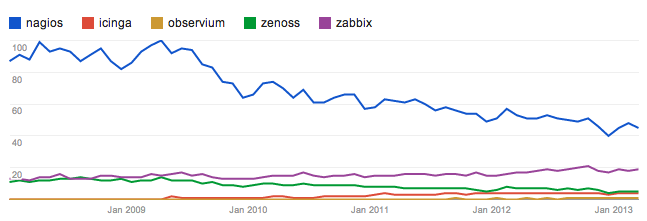
\includegraphics[scale=0.6]{img/monitoring_google_trends}
    \caption{Google Trends: overvåkningsløsninger}
    \label{losninger}
\end{figure}

\section{Valg av kjerneprogramvare}
Valg av kjerneprogramvare var gruppens viktigste valg, da det la grunnmuren for resten av prosjektet, og ville få stor innvirkning på sluttresultatet. Av kandidatene nevnt i \ref{sec:hvilkefinnes}, ble Icinga og Nagios videre vurdert.  

Icingas distribuerte system består av kjernen, som står for prossessering, et databaselag, og administrering av systemet via et webgrensesnitt. Dette er tilrettelagt for et distribuert oppsett. Nagios sin arkitektur har avhengigheter mellom web og lagring av status, som fører til at disse ikke kan separeres. Det er derimot mulig å separere ut MySQL-databasen som Nagios benytter\cite{icingaarchitecture}.

For uthenting av informasjon i Icinga er det utviklet et API som brukes via Icinga Web. Dette gir ett punkt for uthenting av data, med samme oppbygging for alle spørringer. I Nagios er det ikke noen standardisert måte å hente ut informasjon\cite{icingaapi}.

En annen fordel med Icinga er støtte for LDAP-autentisering i Icinga Web, som videre kan benyttes til å styre tilgang til ulik informasjon for brukere. Med Nagios kan en også innføre LDAP-støtte, men dette blir da autentisering via en web-server, og videre kontroll av aksess er ikke mulig. Nagios har noe aksesstyring, men det er bare på et objekt kalt ``contactgroups''. Icinga har aksesstyring på en rekke flere objekter\cite{icingaweb}.

For databaseoppsett støtter Icinga de tre databasemotorene PostgreSQL, Oracle og MySQL. Nagios har bare støtte for MySQL. I oppgavebeskrivelsen er det krav om MySQL, men for fremtidig bruk av Icinga er det mulighet for å benytte de to andre.

Icinga har også en tilleggsmodul kalt ``Icinga Mobile''. Denne gir tilrettelagt grensesnitt for mobile enheter, som var ønsket i oppgavebeskrivelsen. Icinga Mobile kan brukes for å gi et grensesnitt tilpasset mindre skjermer. Ved utsendelse av SMS eller e-post til en eller flere ansatte, kan Icinga-Mobile brukes via samme enhet for å se mer utfyllende informasjon om problemet, samt gjøre administrative handlinger.

Etter en vurdering av denne funksjonaliteten, ble det besluttet å basere overvåkningsløsningen på Icinga framfor Nagios.
\clearpage
\section{Icinga}
For å kunne forstå implementasjonsdelen av prosjektrapporten er det behov for noe innsikt i hvordan Icinga fungerer. I dette delkapittelet er det viktigste forklart.
\subsubsection{Arkitektur}
Icinga består av tre separate komponenter, som vist i Figur \ref{icingacomponents}.

\begin{figure}[H]
    \centering
    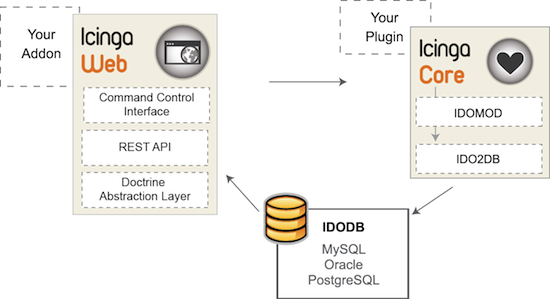
\includegraphics[scale=1.2]{img/icinga_architecture}
    \caption{Icingas tre komponenter}
    \label{icingacomponents}
\end{figure}

\subsubsection{Core}
Icinga Core håndterer planlegging av sjekker gjennom plugin-er og tar i mot resultatene av disse. Denne informasjonen sendes gjennom SSL-krypterte TCP-sockets videre til IDO2DB-prosessen (Icinga Data Out to Database) gjennom et interface kalt IDOMOD (Icinga Data Out Module). Ved å bruke disse abstraksjonslagene kan databasemotoren enkelt byttes ut. I dokumentasjonen er det laget veiledninger for MySQL, PostgreSQL og Oracle\cite{icingaarchitecture}.

IDOMOD og IDO2DB kommer i en samlet pakke (IDOutils), men kan separeres ut for å skape et distribuert oppsett. CERN i Sveits har nylig implementert et slikt oppsett med hjelp av lastbalansereren ``Mod Gearman''\cite{cernthesis}.

\subsubsection{Web}\label{sec:teoriweb}
I utgangspunktet kommer ikke Icinga med noe webgrensesnitt. Men det er mulig å installere to forskjellige pakker for å få dette. I begge kan en få en oversikt over tilstanden til enheter og tjenester, se konfigurasjon og utsendte varsler, samt utføre administrative oppgaver. Det kan også hentes ut statistikk over oppe- og nedetid.

Icinga Classic baserer seg på det samme vindusoppsettet som Nagios. For uthenting av data benyttes CGI-moduler som henter ut data fra filen ''status.dat''. Filen blir brukt av Icinga for å lagre tilstandsinformasjon om enheter og tjenester, kommentarer, og informasjon om nedetid. 

Icinga Web er en total omskrivning av webgrensesnittet. Det er en Ajax-drevet, Web 2.0-inspirert front-end, som har flere lag mellom kjernen av Icinga og visningene:

\textbf{Doctrine Abstraction Layer} henter informasjon fra databasen. Det kan også benyttes av utviklere for å legge til egne moduler i Icinga Web med uthenting av informasjon fra andre databaser.
\textbf{REST API} presenterer dataene fra DAL til Icinga Web. Her kan autentisering utføres slik at en kan sette hvilken informasjon ulike brukere skal kunne se.
\textbf{Command Control Interface} kan videresende kommandoer til Icinga Core. For eksempel manuell kjøring av en sjekk eller restart av Icinga. 

\section{Objekter}\label{sec:objekter}
All konfigurasjon av Icinga gjøres i tekstfiler. I selve konfigurasjonsfilen ''icinga.cfg'' settes filbanen til konfigurasjonsfilene. Icinga vil da ved oppstart lete rekursivt gjennom mappen etter filer som ender med ''.cfg''.

Konfigurasjonsdataene er bygget rundt det som i Icinga kalles objekter. Dette er en samling av konfigurasjon som hører sammen. Selv om en ikke kan si at Icingas objekter er det samme som objekter i programmeringsverden, benyttes mange av de samme begrepene og konseptene.

En rekke objekter er definert i Icinga, som vist i Tabell \ref{objekter}.

\begin{changemargin}{-1cm}{-1cm}
\begin{table}
\begin{center}
%\begin{tabular}{|p{2.0in}|c|c|c|} \hline
\begin{tabular}{ | p{3.5cm} | p{6.5cm} | p{6cm} |} \hline
	\textbf{Objekt} & \textbf{Forklaring} & \textbf{Eksempel} \\ \hline
	Host & En enhet med en adresse (typisk IP-adresse eller MAC-adresse). & Server, switch, router etc. \\ \hline
	Command & En kommando som skal kjøres på overvåkningsserveren & Et program, for eksempel check\_ping. \\ \hline 
	Service & Kombinasjonen av et host-objekt og et command-ojekt. & Sjekk oppetid: kommandoen ``check\_uptime'' skal kjøres på ``dc1''. \\ \hline
	Servicegroup & Service-objekt knyttet til host-objekter satt sammen til en applikasjon. & En applikasjon har tre prosesser som må være kjørende for at applikasjonen fungerer. Disse grupperes under samme servicegroup. \\ \hline
	Contact & Når og hvordan en person skal kontaktes angående en service. & Jens skal få en SMS hvis DHCP ikke er tilgjengelig. \\ \hline
	Timeperiod & Navn og definisjon av en tidsperiode. & Mellom 08.00 og 16.00 på annenhver tirsdag, hvis det er den tredje dagen i måneden. \\ \hline
	Host dependency & En eller flere avhengigheter. Dersom et host-objekt er avhengig av et annet, og det ikke svarer lenger, trenger ikke Icinga utføre sjekker på det avhengige objektet. & kantswitch1 er avhengig av kjerneswitch. \\ \hline
	Service dependency & Samme som host, men for service. & Captive portal er avhengig av RADIUS. \\ \hline
	Host escalation & Hva skal skje etter at en host har vært nede etter en definert tid. &	Om dc1 har vært nede i 30 minutter, send e-post til Ola Sysadmin. Etter 60 minutter sendes SMS til alle i admin contactgroup-en \\ \hline
	Service escalation & Samme som for objektet host-dependency, men for service-objeker. & Om DNS har vært nede i 30 minutter, send e-post til Kari Sysadmin. Etter 60 minutter send SMS til alle i admin hostgroup-en. \\ \hline
	\end{tabular}
	\caption{Oversikt over objekter i Icinga}
	\label{objekter}
\end{center}
\end{table}
\end{changemargin}

I tillegg til disse kan host, service og contact grupperes med henholdsvis hostgroup, servicegroup og contactgroup.

Det er også to objekter med metainformasjon, ``hostextinfo'' og ``serviceextinfo'', der en kan definere ekstra konfigurasjon som bildebaner, notater og koordinater for host- og service-objekter.

Den siste objekttypen er module. Her spesifiseres konfigurasjon for en modul som utvider funksjonalitet i Icinga Web.

Sammenhengen mellom objektene er viktig å forstå for å skjønne hvordan sjekker utføres i Icinga. I et service-objekt defineres hvilket command-objekt som skal benyttes for å teste tjenesten og hvilke host- eller hostgroup-objekter dette skal sjekkes på. Dette er vist i Figur \ref{command_host_service}.

\begin{figure}[H]
    \centering
    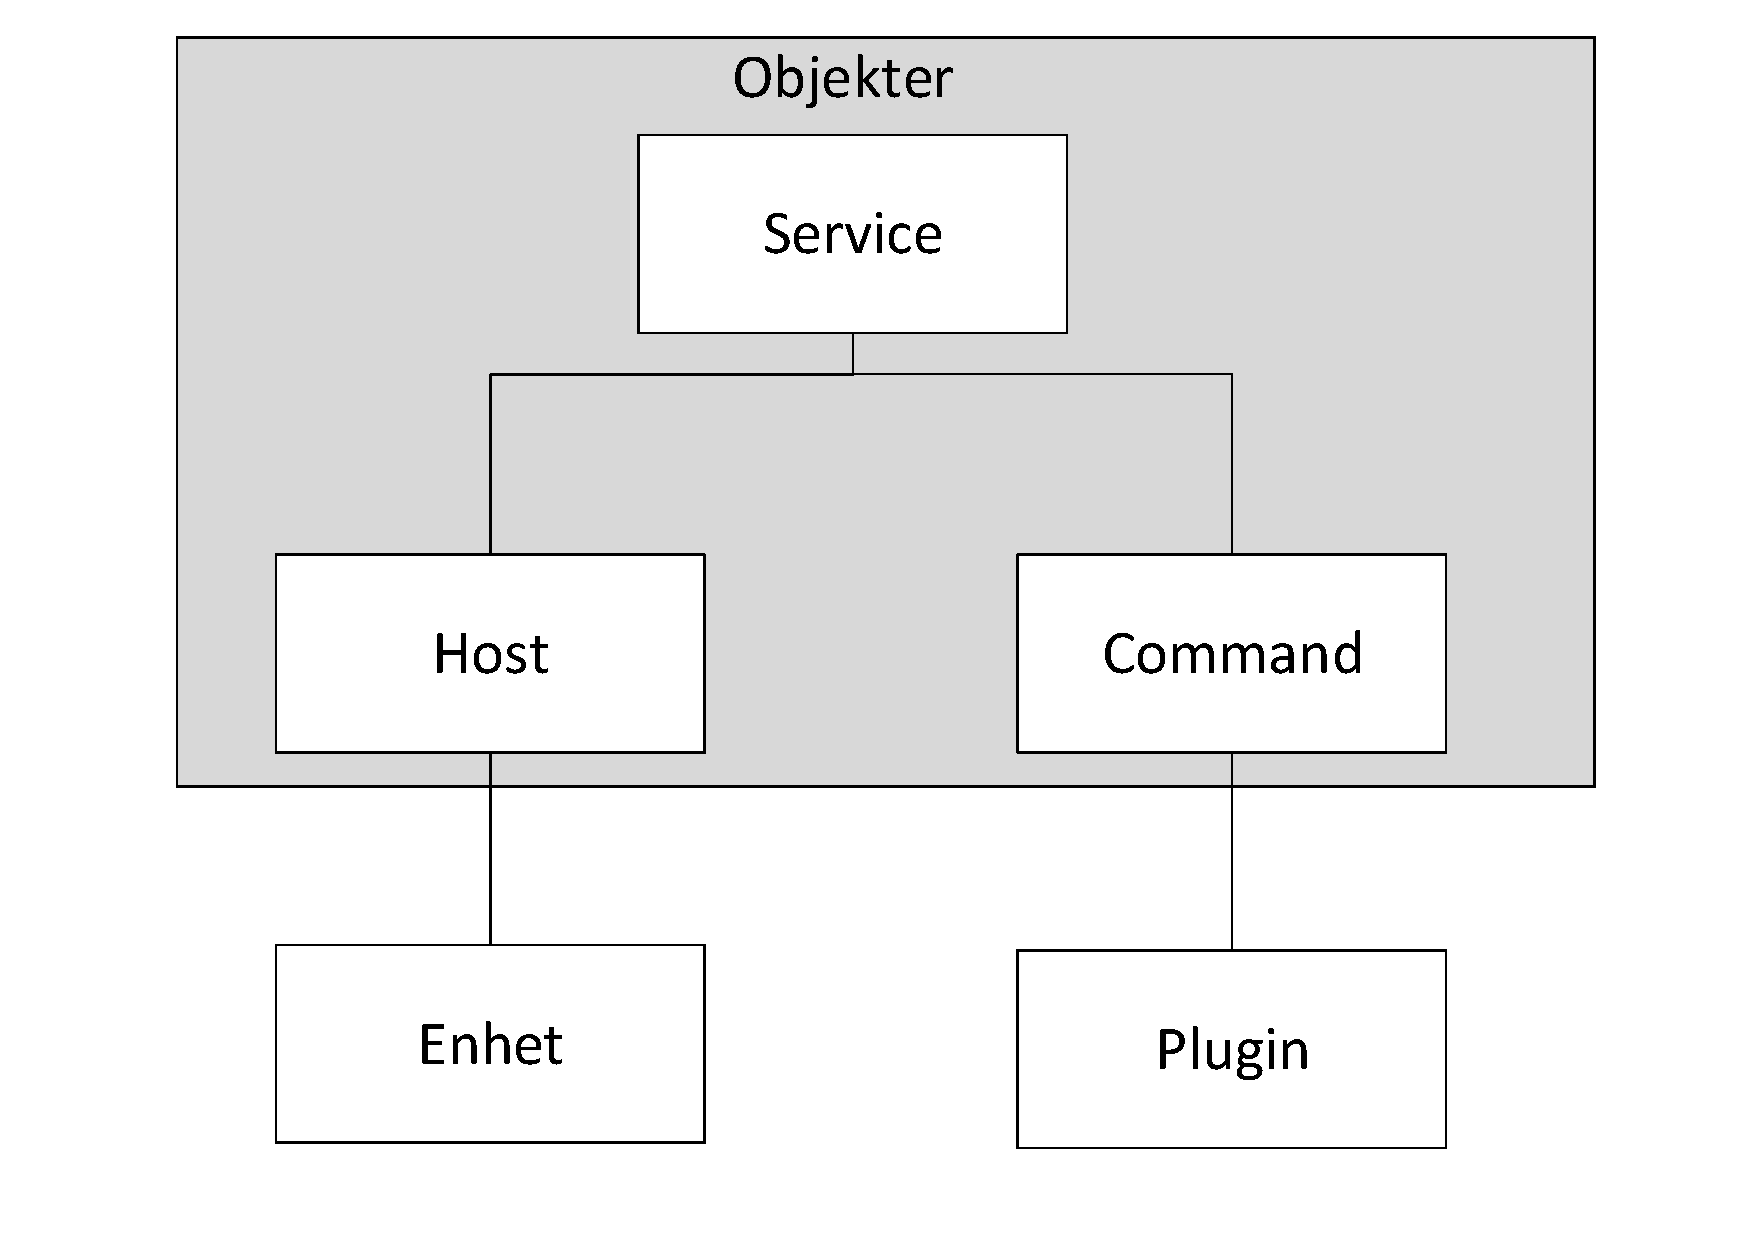
\includegraphics[scale=0.4]{img/command_host_service}
    \caption{Sammenhengen mellom host-, service- og command-objekter.}
    \label{command_host_service}
\end{figure}
% Si noe om utelatt konfig, arv ved use?
I eksempelet under vises konfigurasjonen for å sette opp en ping-sjekk på HiG1.
\begin{lstlisting} [style=example]
define host {
    use                  generic_host
    host_name            HiG1
    address              192.168.0.1
}

define service {
    use	                 generic_service
    host_name            HiG1
    service_description  Ping
    check_command        check_ping!200,5%!500,10%
    check_interval       5
}

define command {
    command_name         check_ping
    command_line         /usr/lib/nagios/plugins/check_ping -H $HOSTADDRESS$ --warning $ARG1$ --critical $ARG2$   
}
\end{lstlisting}

\clearpage
\section{Plugin-er}
Icinga i seg selv kommer uten noen overvåkningssjekker. Til dette benyttes plugin-er.

En plugin i Icinga er et eksternt program som kjøres og outputen hentes inn som data. Resultatet av sjekken hentes fra exit-koden\cite{wiki:returncode} og oversettes til en tilstand, som vist i Tabell \ref{state}.

En plugin kan være noe helt enkelt som scriptet under. Der exit-koden til en ping-kommando sjekkes. Hvis ping ikke får svar, vil den gi exit-koden 1. Scriptet vil da gi exit koden 2, som i Icinga oversettes til CRITICAL.
\begin{lstlisting}[language=bash]
#!/usr/bin/env bash
loss=$(ping -c 5 google.com)
if [ $? -eq 0 ]; then
    echo "OK"
    exit 0
else
    echo "ERROR"
    exit 2
fi
\end{lstlisting}

Det finnes et sett med offisielle plugin-er til Nagios; nagios-plugins, som utgis av ``Nagios Plugins project''. Pakken finnes i en rekke pakkebehandlere og inneholder over 50 plugin-er som er ment for å dekke et grunnleggende overvåkningsbehov\cite{nagiosplugins}.

\begin{table}[H]
	\begin{center}
	\begin{threeparttable}
	\begin{tabular}{| l | l | l |} \hline
	\textbf{Returkode fra plugin} & \textbf{Service-tilstand} & \textbf{Host-tilstand} \\ \hline
	0 & OK & UP \\ \hline
	1 & WARNING & UP eller DOWN/UNREACHABLE* \\ \hline
	2 & CRITICAL & DOWN/UNREACHABLE \\ \hline
	3 & UNKNOWN & DOWN/UNREACHABLE \\ \hline
	\end{tabular}
	\begin{tablenotes}
	\small
	\item *Ved bruk av Aggressive host checking\cite{icingapluginapi}.
	\end{tablenotes}
	\caption{Tilstandsoversikt}
	\label{state}
	\end{threeparttable}
	\end{center}
\end{table}

\section{Sjekker}\label{sec:sjekker}
Tilstanden for et service- eller host-objekt vil bestemmes ut i fra et returnert resultat fra en aktiv eller passiv sjekk. Forskjellen på disse to vil bli forklart i de neste delkapitlene.

Dersom en aktiv eller passiv sjekk resulterer i en annen tilstand enn OK, er det to typer av tilstanden, ``SOFT'' og ``HARD''. Første gang en plugin returnerer en feil vil tilstanden bli satt til SOFT, i tillegg til service- eller host-tilstanden. Etter dette vil sjekken kjøres hyppigere for å finne ut om det er snakk om et forbigående problem. Etter et gitt antall ganger der plugin-en fortsatt ikke returnerer OK, vil tilstanden skifte til HARD og det sendes ut varslingsmelding. Varsling er beskrevet grundigere i \ref{sec:varsling}.

\clearpage
\subsubsection{Aktive sjekker}
En aktiv sjekk er en sjekk som initieres av Icinga, der en kommando kjøres på Icinga-serveren. Dette er også kjent som en ``poll''-modell. En aktiv sjekk defineres ut i fra et command-objekt med parametere og et tidsintervall i service- og host-objekter. I command-objektet defineres en plugin som skal kjøre, og returverdien fra denne vil bestemme hvilken tilstand service- eller host-objektet har. I Figur \ref{active_checks} vises komponentene involvert i en aktiv sjekk.
\begin{figure}
   \centering 
   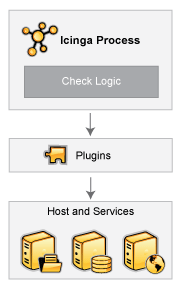
\includegraphics[scale=0.7]{img/activechecks.png}
    \caption{Aktive Sjekker}
    \label{active_checks}
\end{figure}

\subsubsection{Passive sjekker}
Passive sjekker går motsatt vei av aktive sjekker. Her vil hver host si ifra når verdier har overgått en satt grense eller en feil har oppstått. Dette kalles ofte for en ``push''-modell. Passive sjekker kjøres ved at et eksternt program skriver en linje med informasjon om tjenesten og sjekkresultat til en fil, som Icinga sjekker periodisk. Dette er illustrert i Figur \ref{passive_checks}.

Fordelen med passive sjekker er at Icinga vil oppdage feil raskere. Ved standard konfigurasjon sjekkes filen med sjekkresultater så ofte som mulig, mens aktive sjekker kjøres hver 5. minutt. Passive sjekker vil også avlaste Icinga-serveren, da alle sjekker utelukkende vil bli kjørt lokalt på enheten som overvåkes. Men en må åpne for at kommunikasjon kan initieres fra alle enheter som skal overvåkes til Icinga-serveren, og mister da samtidig muligheten til å samle all konfigurasjon på ett sentralt sted. 

\begin{figure}[H]
    \centering
    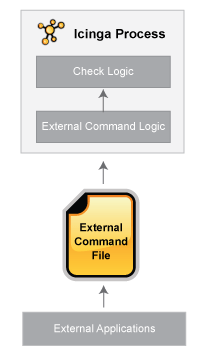
\includegraphics[scale=0.7]{img/passivechecks.png}
    \caption{Passive Sjekker}
    \label{passive_checks}
\end{figure}

\subsubsection{Hostsjekk}
Resultatet av en host-sjekk vil avgjøre om tilstanden til host-objektet er ``UP'' eller ``DOWN''. 

Det er ikke et fast tidsintervall for en hostsjekk med mindre check\_interval er definert for objektet. Icinga vil kjøre sjekken om en service som er satt opp for host-en skifter tilstand. Service-objekter som er definert for en host som er i ``DOWN'' vil automatisk bli vist under ``Known service problems'' i webgrensesnittet, og ingen sjekker vil bli kjørt på dem før host-en er ``OK'' igjen.

Grunnsjekken for en host defineres i host-konfigurasjonen med ''check\_command'', som vist under.
\begin{lstlisting}[style=example]
define host {
...
    check_command	check_host_alive
}
\end{lstlisting}

\subsubsection{Variabler}
For å kunne gjøre konfigurasjon av Icinga mest mulig dynamisk er det en rekke forhåndsdefinerte variabler en kan bruke i konfigurasjonsfilene. Disse kalles makroer. En fullstendig liste over disse og hvor de kan benyttes finnes i Icinga-dokumentasjonen\cite{icingamacro}. ''\$HOSTADDRESS\$'' kan for eksempel benyttes i et command-objekt slik at det bare må skrives en gang, og ikke for hver host. En kan også definere egne variabler som for eksempel ''\_SSHPORT''. Disse kan sendes videre til selve kommandoen som kjøres og benyttes som argumenter til plugin-en som kjører en sjekk, slik:
\begin{lstlisting}[style=example]
define host {
...
    host_name		example_server
    _SSHPORT		222
}
define command {
    command_name	check_ssh
    command_line	$USER1$/check_ssh -H $HOSTADDRESS$ -p $_HOSTSSHPORT$
}
\end{lstlisting}

Her benyttes de innebygde variablene ``USER1'' for banen til plugin-en som kjøres, HOSTADDRESS for IP-en til den hosten som sjekken skal kjøres på og den egendefinerte variabelen \_SSHPORT som defineres på host-objektet.

USER-variablene defineres i den globale konfigurasjonsfilen og brukes der hvor informasjon skal sjules fra webgrensesnittet. Som for eksempel når det trengs et passord for å utføre en sjekk.

\subsubsection{Templates}
En template er ikke et objekt i seg selv, men en mal for et objekt. Med direktivet ``register 0'' vil ikke Icinga registrere dette objektet for overvåkning. Ved å bruke direktivet ``use'' kan en i et annet objekt ``arve'' konfigurasjonen fra template-en. Template-er kan også arve, og en kan dermed sette opp et hierarki der en spesifiserer generell konfigurasjon i toppen og arver nedover til mer spesiell. 

I eksempelet under er generell konfigurasjon for alle host-objekter definert i ``generic\_host'', som brukes i de andre objektene. I ``generic\_firewall'' erstattes verdien for kontaktgruppe, og i cisco\_firewall settes en egendefinert variabel:

Template-en generic\_host: 
\begin{lstlisting}[style=example]
define host {
    name                            generic_host    ; The name of this host template
    notifications_enabled           1       ; Host notifications are enabled
    event_handler_enabled           1       ; Host event handler is enabled
    flap_detection_enabled          1       ; Flap detection is enabled
    failure_prediction_enabled      1       ; Failure prediction is enabled
    process_perf_data               1       ; Process performance data
    retain_status_information       1       ; Keep status after Icinga restart
    retain_nonstatus_information    1       ; Keep non-status after Icinga restart
    check_command                   check-host-alive
    max_check_attempts              10
    normal_check_interval           5
    retry_check_interval            2
    notification_interval           0
    notification_period             24x7
    notification_options            d,u,r
    contact_groups                  all_contacts
    register                        0       ; Not a real host, just a template
}
\end{lstlisting}

Template-en generic\_firewall, som arver fra generic\_host:
\begin{lstlisting}[style=example]
define host {
   name             generic_firewall
   use              generic_host
   contact_groups   firewall_admins
   register         0
}
\end{lstlisting}

Template-en cisco\_firewall, som arver fra generic\_firewall:
\begin{lstlisting}[style=example]
define host {
    name            cisco_firewall
    use             generic_firewall
    register        0
    _WANPORT        WAN ; Custom variable for WAN port to monitor
}
\end{lstlisting}

Host-objektet hig-hw1, som arver fra cisco\_firewall:
\begin{lstlisting}[style=example]
define host {
    use             cisco_firewall
    host_name	    hig-fw1
}
\end{lstlisting}

Dette gjør at det blir lite konfigurasjon hver gang en ny brannmur skal legges til.

\subsubsection{Regulære uttrykk}
Ved å sette ``use regular expressions'' i konfigurasjonen for Icinga, kan en benytte regulære uttrykk i attributter i et objekt, der en refererer til andre objekter. Icinga støtter standarden POSIX Extended Regular Expressions, og vil automatisk tolke navnet på objekter som et regulært uttrykk dersom det inneholder \verb|"*", "?", "+", eller "\"|.

Dette kan være nyttig dersom en for eksempel vil legge alle hoster i en hostgroup, som har en navnekonvensjon som gjør at hver av hostene unikt kan identifiseres ved å bytte ut deler av navnet med en variabel.

I eksempelet nedenfor brukes det regulære uttrykket \verb|"^HiG\[0-9\]+\$"| i attributten ``members'' til å legge til alle konfigurerte hosts der navnet starter på ``HiG'' etterfulgt og avsluttet med ett eller flere siffer mellom 0 og 9, i hostgroup-objektet ``all\_servers''.
\begin{lstlisting}[style=example]
define hostgroup {
    hostgroup_name	all_servers
    alias		All Servers
    members		^HiG[0-9]+$
}
\end{lstlisting}

Det kan også benyttes til å ekskludere en host fra en service-sjekk. I eksempelet nedenfor er HiG3 medlem av hostgroup-en ``windows\_servers'', men blir ekskludert fra å kjøre sjekken på diskplass ved å sette ``!HiG3'':
\begin{lstlisting}[style=example]
define service {
    use				generic_service
    service_description		Disk space
    hostgroup_name		windows_servers
    host_name			!HiG3
    check_command		win_nrpe!CheckDriveSize!Drive="C" MaxWarnUsed=80% MaxCritUsed=90%
}
\end{lstlisting}

\section{Avhengigheter}
I Icinga kan en definere tre ulike typer avhengigheter, ``Parent'', ``Service dependency'', og ``Host dependency''. Disse har innvirkning på hvilke varsler som sendes ut og statusen de ulike service- og host-objektene får. Hver av disse krever egen konfigurasjon. 

\section{Parent}\label{sec:parent}
Et host-objekt kan settes som en parent til et annet host-objekt. Host-objekter som har en parent blir betegnet som en child-host eller child-service. Dette brukes primært for å unngå varsler om andre host- og service-objekter enn det som er definert som parent, om denne blir utilgjengelig. For eksempel hvis kjernerouteren mister strømtilgangen, ønskes ikke varsler for eventuelle host-objekter og tilhørende service-objekter som har kjernerouteren som parent. Disse vil ikke lenger bli sjekket og tilstanden vil bli satt til ``UNREACHABLE''. Tjenester som tilhører host-ene vil få tilstanden ``UNKNOWN''.

For redundante oppsett kan et host-objekt ha flere ``parents'' definert. Host-objektet vil da ha tilstanden UP så lenge minst én ``parent''-host er UP.

Ut ifra parent-relasjonene mellom host-objekter i konfigurasjonsfilene genereres også et ``Status Map'' over nettverket, som vist i Figur \ref{statusmap}. Dette brukes til å visualisere alle relasjonene, og vil gjengi redundante oppsett og hvilke host-objekter som er påvirket av at parent-hosten er DOWN.

\begin{figure}[H]
    \centering
    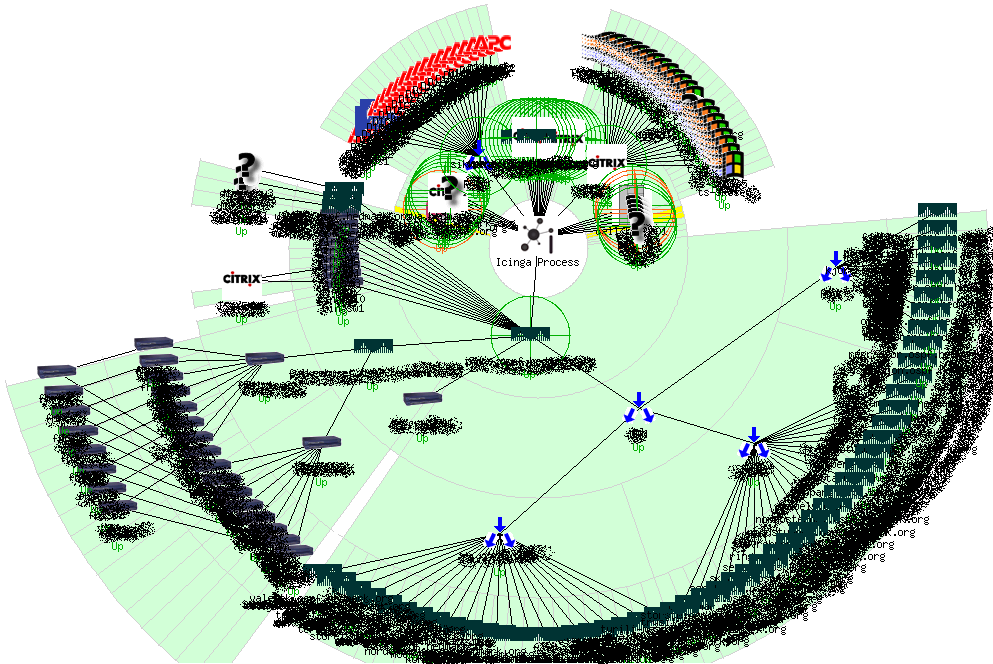
\includegraphics[scale=0.6]{img/statusmap}
    \caption{Kart som viser parent- og host-relasjoner}
    \label{statusmap}
\end{figure}

\section{Service dependency}\label{sec:servicedependency}
Service dependency er en egen objekttype der en kan sette opp avhengighet mellom to service-objekter. Formålet med dette er å unngå varsel hvis en tjeneste får tilstanden DOWN, som følge av at en annen tjeneste har det. For eksempel bør det ikke varsles om at tjenester som er avhengig av autentisering via LDAP-serveren får ``Access Denied''-feilmeldinger, hvis LDAP-serveren er DOWN. Det service-objektet andre service-objekter er avhengige av kalles en master service. 

Icinga undersøker om avhengigheter er definert for et service-objekt, før det utføres sjekker på det. Dette er med på å bestemme om det blir sendt ut varsel for service-objektet.

I eksempelet under er tjenesten ``Check SMB'' på HiG3 avhengig av master-service-en Check LDAP på HiG3. ``execution\_failure\_criteria'' bestemmer ved hvilke tilfeller tjenesten ikke skal sjekkes. Her er den satt til ``c'', som vil si at Check SMB ikke skal kjøres dersom ``Check LDAP'' er i CRITICAL tilstand.

\begin{lstlisting}[style=example]
define servicedependency {
    host_name                          HiG3
    service_description                Check LDAP
    dependent_host_name                HiG3
    dependent_service_description      Check SMB
    execution_failure_criteria         c
    notification_failure_criteria      c
}
\end{lstlisting}

Ved standard konfigurasjon vil Icinga benytte siste harde tilstand for master service. Dersom ``max\_check\_attempts'' for eksempel er satt til 4, vil ikke Check SMB stoppes fra å kjøres før Check LDAP har blitt sjekket fire ganger, og oppnår en hard tilstand. 

På attributten notification\_failure\_criteria kan det settes hvilke service-tilstander en ikke skal varsle for. Dette er hovedgrunnen til at det settes opp slike avhengigheter. Når denne er satt til ``c'' vil det ikke varsles om master service-en får tilstanded CRITICAL.

Service-objekter har kan også arve avhengighetene til en master service ved å sette direktivet ``inherits\_parent 1''. For eksempelet over vil Check SMB da arve fra service-objekter som Check LDAP arver fra.

For å konfigurere avhengigheter mellom tjenester som kjører på samme host kan en utelate ``dependent\_host\_name'' I eksempelet under vil alle tjenester på host-objektet være avhengig av tjenesten ``NRPE-daemon''.

\begin{lstlisting}[style=example]
define servicedependency{
    ;dependent_host_name   	    ; Not defined to make dependancy on same host            
    hostgroup_name 		    linux_servers
    service_description             NRPE-daemon
    dependent_service_description   NRPE Check *
    execution_failure_criteria      c
    notification_failure_criteria   c
}
\end{lstlisting}

En kan også erstatte host\_name og dependant\_host\_name med hostgroup og dependant\_host\_group for å lage avhengigheter på alle objekter som tilhører gruppen.

\section{Host dependency}
For å sette en avhengighet mellom to host-objekter benyttes host dependency. Dette må ikke forveksles med parent, som refererer til nettverksoppsettet. En host dependency vil si at et host-objekt er avhengig av et annet host-objekt. Host dependency er bare nyttig i veldig spesielle tilfeller, da det for de fleste tilfeller vil være avhengigheter til en eller flere tjenester på host-en\cite{hostandservicedep}, eller at en host er avhengig av å kjøre en sjekk igjennom en annen host.

\section{Protokoller og agenter}
For å kjøre sjekker på enheter må Icinga-serveren kunne kommunisere med operativsystemene på de ulike enhetene. Icinga henviser til protokollene SSH, SNMP, RPC (WMI) og agentene NRPE og NSCA (en del av pakken NSClient++) i dokumentasjonen\cite{icingaintegration,icingaadditionalsoftware}. 

\subsubsection{NRPE}\label{sec:nrpe}
NRPE (Nagios Remote Plugin Executor) består av plugin-en ``check\_nrpe'' på Icinga-serveren og en daemon som installeres på hver server som skal overvåkes. NRPE eksekverer lokale plugin-er på den eksterne serveren og returner dataen fra denne til check\_nrpe. Tillatelse for eksekveringer defineres i en konfigurasjonsfil på hver server, der en oppgir hvilke IP-adresser som kan koble seg til og hvilke kommandoer som er gyldige. 

\begin{figure}[H]
    \centering
    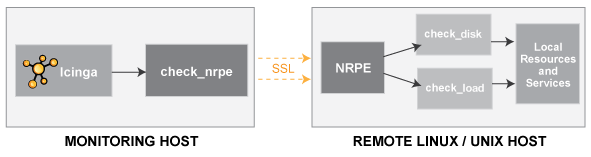
\includegraphics[scale=0.6]{img/nrpe.png}
    \caption{NRPE}
    \label{nrpe}
\end{figure}

\subsubsection{SSH}
Gjennom en tilkobling til en SSH (Secure Shell)-server kan en spesifisere en kommando som skal kjøres på en ekstern maskin, og hente output-en til det opprinnelige shellet. Dette virket som den beste måten å overvåke Linux-servere på, ved starten av prosjektet. SSH-prosjektet er meget utbredt og blir aktivt sjekket for sikkerhetshull. SSH er også installert på de aller fleste Linux-servere, og en vil dermed unngå å lytte på en ekstra port.

Ulempen med å kjøre sjekker over SSH er at en må sette opp nøkkelbasert innlogging mellom Icinga-serveren og alle Linux-serverne som skal overvåkes. En kan begrense rettigheter for brukeren som kjører sjekkene, men den vil fortsatt ha muligheten til å logge inn til et shell og eksekvere kommandoer. Dette kan føre til at en potensiell angriper via Icinga-serveren, har en vei inn til alle servere som overvåkes, ved å bruke den private nøkkelen.

SSH gir også endel overhead både på nettverkstrafikk og i CPU-tid\cite{sshmanpage}. En måte å begrense dette på er å benytte SSH med ControlMaster. Dette innebærer en endring i SSH-konfigurasjonen på serveren, slik at SSH-klienten lagrer informasjon om hver utgående TCP-tilkobling, og samme tilkobling kan benyttes mot samme host. Dermed unngås en ny TCP-tilkobling for hver ny sjekk som skal utføres på hosten.

\subsubsection{SNMP}
Det meste av nettverksutstyr beregnet for bedrifter, har i dag støtte for protokollen SNMP (Simple Network Management Protocol\cite{essentialsnmp}). SNMP definerer en enkel og effektiv måte å overvåke enheter på og det gir en standard som leverandørene følger.
	
SNMP baserer seg på variabler som blir gjort tilgjengelig på enheten som skal overvåkes (kalt agenten). Disse variablene er definert i en Management Information Base (MIB). MIB-filene er ofte tilgjengelige på produsentens hjemmeside. Her beskrives strukturen for dataen i et hierarkisk navnerom som inneholder Object Identifier (OID). Hver OID identifiserer en variabel som kan bli lest eller satt via SNMP. Enheten som ber om disse variablene kalles ``manager''. 

En ulempe med SNMP er at OID-ene er lange og tunge å lese. For eksempel for å hente ut batterikapasiteten på en APC UPS benyttes OID-en:
\
1.3.6.1.4.1.318.1.1.1.2.2.1.0
\
Dette kan oversettes til:
\
iso(1). org(3). dod(6). internet(1). private(4). enterprises(1). apc(318). products(1). hardware(1). ups(1). upsBattery(2). upsAdvBattery(2) upsAdvBatteryCapacity.0
\
Denne OID-en er definert i APCs MIB-fil ``PowerNet MIB''. Ved å laste inn denne kan en også benytte ``PowerNet-MIB::upsAdvBatteryCapacity.0''.

SNMP finnes i flere versjoner. I dag brukes for det meste versjon 2c og den nyeste, versjon 3. De ulike versjonene er ikke kompatible, men i praksis støtter det meste av utstyr som støtter v3 eller v2c også v1 \cite{rfc3584}. Hovedforskjellen på versjon 2c og 3 er at versjon 3 har støtte for flere sikkerhetsmekanismer, men krever noe mer konfigurasjon. Sikkerhetsaspektet ved dette er diskutert videre i Kapittel \ref{chap:sikkerhet}.

Det eksisterer to muligheter når enheter skal overvåkes via SNMP. Enten kan enhetene selv rapportere inn hendelelser via SNMP trap/inform, eller så kan serveren spørre enhetene via SNMP GetRequest. Valg av det første medfører at en kan gjøre varsling umiddelbart, men da må også hver enhet konfigureres med parametere for hvilke trap-meldinger som skal sendes og til hvilken IP-adresse. Icinga har ingen støtte for å motta trap-er, men en kan installere en egen daemon for dette og rapportere inn data med passive sjekker. 

For å benytte SNMP trap/inform må en tillate tilkoblinger til overvåkingsserveren i stedet for bare fra denne. Hvilke trap-meldinger som skal sendes må også konfigureres på hver enhet, og en vil da ikke kunne ha alle konfigurasjoner sentralisert på Icinga-serveren.

\begin{figure}[H]
    \centering
    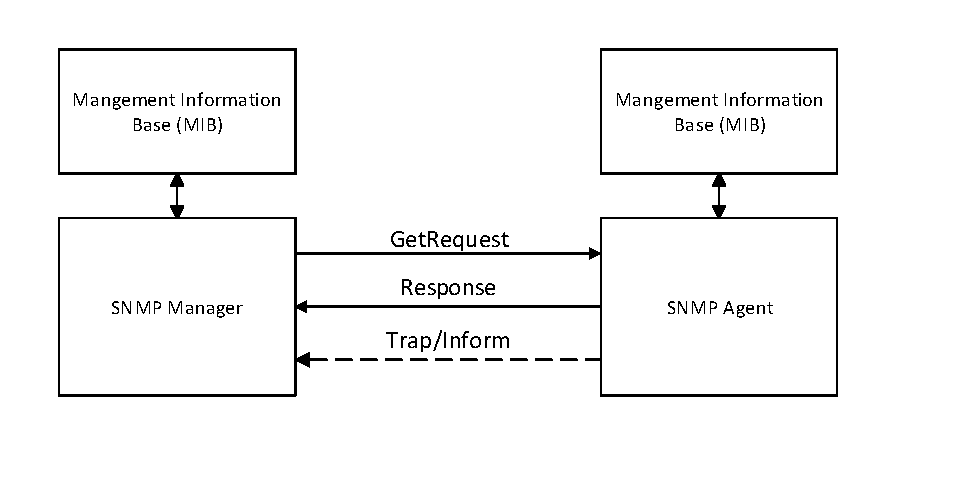
\includegraphics{img/SNMP}
    \caption{Overvåkning med SNMP}
    \label{SNMP}
\end{figure}

SNMP benytter seg av UDP for å levere trap-meldinger. UDP er en såkalt upålitelig protokoll, noe som vil si at det ikke er noen omsending av pakker eller noen tilbakemelding (ack) for at pakkene kommer fram. Derfor kan en risikere å miste en trap. SNMP inform, som kom i SNMPv3, løser dette ved at agenten vil sende en ny inform-pakke i et intervall, helt til manageren gir beskjed om at trap-meldingen er mottatt.

For å benytte SNMP på Windows- og Linux-servere kreves installasjon av en SNMP-agent\cite{mssnmp,netsnmp}.

\subsubsection{WMI (Windows Management Instrumentation)}
WMI er et grensesnitt som gjør det mulig å lage programmer eller script som utfører oppgaver mot operativsystemet Windows, både lokalt eller på eksterne maskiner. Disse oppgavene kan være alt fra å restarte maskinen, til å hente ut logger over hendelser som har inntruffet på maskinen. I en overvåkningsløsning vil det være mest relevant å kjøre kommandoer som henter ut informasjon om maskinen og tjenester som kjører på den. Dette kan for eksempel være hvilke prosesser som bruker mest CPU-tid.

For å benytte WMI-spørringer direkte fra en ekstern enhet må det konfigureres brukertilgang og brannmurregler\cite{wmiremote}. Med NSclient++ har en mulighet til å kjøre WMI-spørringer over NRPE uten ekstra konfigurasjon.

\subsubsection{Valg av Agenter}
Valg av protokoll eller agenter har basert seg på følgende punkter:
\begin{itemize*}
	\item Ressursbruk (CPU)
	\item Nettverkstrafikk
	\item Utrulling
	\item Sikkerhet
\end{itemize*}
Nettverkstrafikken som ble generert ved både en NRPE- og en SSH-sjekk ble målt ved å benytte et Bash-script som kjørte en disk-sjekk 100 ganger, som vist under. 

\begin{lstlisting}[style=example,language=bash]
#!/usr/bin/env bash
if [ "$1" == "ssh" ]; then
    cmd="/usr/lib/nagios/plugins/check_by_ssh -H 10.60.0.21 -C \"/usr/lib/nagios/plugins/check_disk -W 10% -C 5% -M -A\" > /dev/null"
elif [ "$1" == "nrpe" ]; then
    cmd="/usr/lib/nagios/plugins/check_nrpe -H 10.60.0.21 -c check_all_mounts -a 10,5 > /dev/null"
else
    echo "You must specify ssh or nrpe as the first argument"
    exit 1
fi
for i in {1..100}; do
    eval $cmd
done
exit 0
\end{lstlisting}

Både serveren og klienten stod i et eget nettverk i Virtualbox sammen med en Windows-maskin med et nettverkskort satt i promiscious mode, for å kunne sniffe nettverkstrafikken. Denne fanget nettverkstrafikken med Wireshark. Trafikken mellom de to maskinene ble hentet ut og data for hver tilkobling ble brukt til å kalkulere båndbreddebruk.

Det ble også undersøkt hvor mye CPU-tid NRPE og SSH trenger for å utføre sjekker. Fordi hver sjekk går veldig raskt ble det kjørt 100 disksjekker, 100 ganger. ``time''-kommandoen ble brukt for å se på tiden brukt i user- og kernel-mode. Dette ble gjort ved å bruke Bash-scriptet nedenfor, som kjører det samme scriptet som ble brukt for å generere nettverkstrafikk.

\begin{lstlisting}[style=example]
#!/usr/bin/env bash

args=(nrpe ssh)

for arg in "${args[@]}"; do
        for i in {1..100}; do
                /usr/bin/time -f "%U\t%S" run_check.sh $arg
        done
done
exit 0
\end{lstlisting}

\begin{figure}[H]
    \centering
    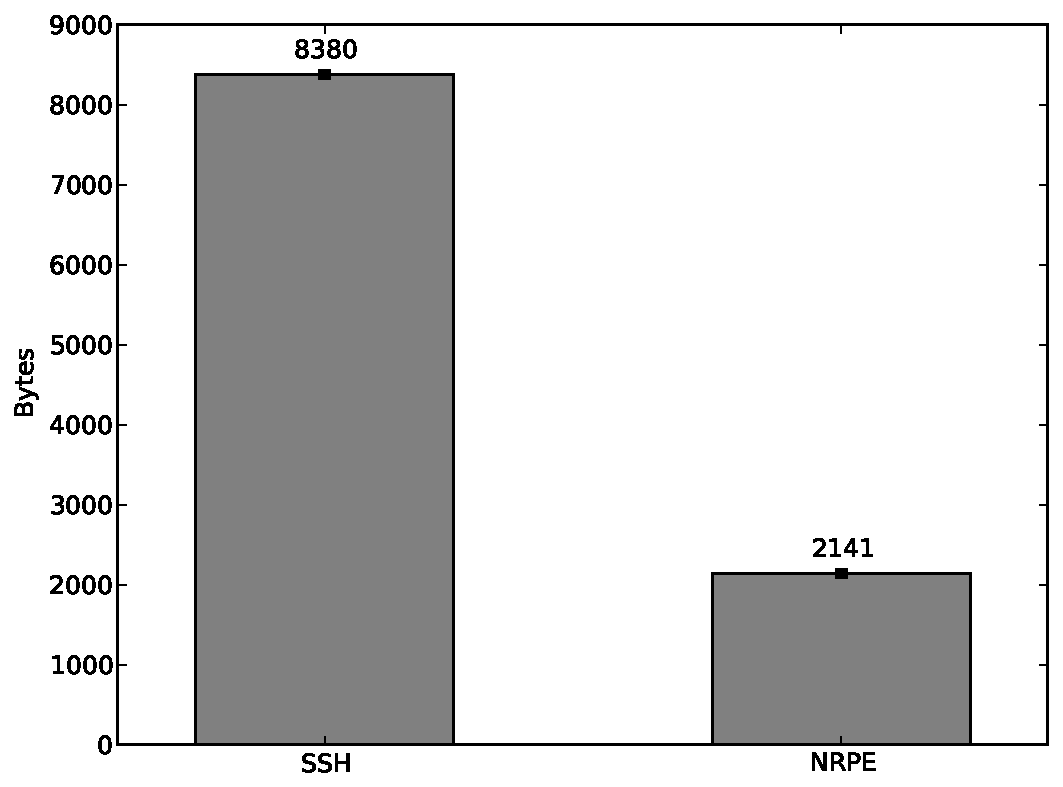
\includegraphics[scale=0.6]{img/nettverkstrafikk}
    \caption{Nettverkstrafikk}
    \label{network_traffic}
\end{figure}

\begin{figure}[H]
    \centering
    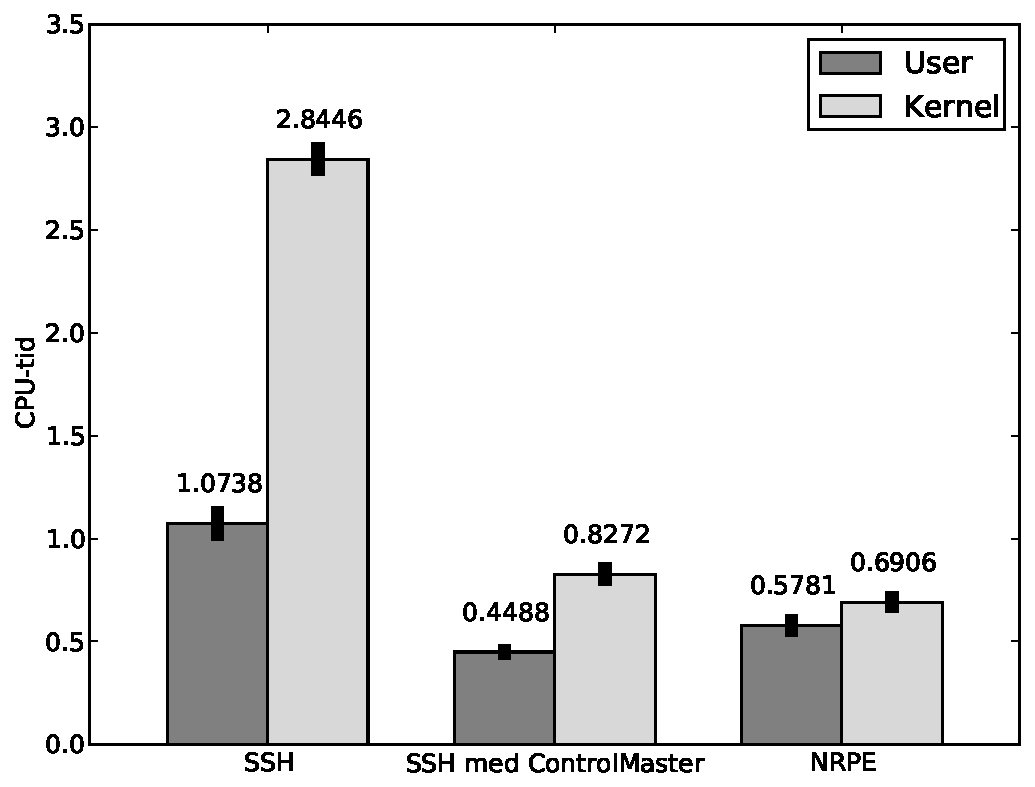
\includegraphics[scale=0.6]{img/cpubruk}
    \caption{CPU-bruk}
    \label{cpu_usage}
\end{figure}

\begin{table}
    \begin{center}
	\begin{threeparttable}
    \begin{tabular}{| l | l | l | l |} \hline
	\ & \textbf{CPU-tid i user(s)} & \textbf{CPU-tid i kernel(s)} & \textbf{Nettverkstrafikk (B)} \\ \hline
	SSH & 1.0738 (0.0792) & 2.8446 (0.0771) & 8380 (101.38) \\ \hline
	NRPE & 0.5781 (0.0347) & 0.6906 (0.0495) & 2141 (55.08) \\ \hline
	SSH med ControlMaster & 0.4488 (0.0509) & 0.8272 (0.0543) & 1700* \\ \hline
	\end{tabular}
	\begin{tablenotes}
	\small
	\item *For SSH med ControlMaster var det ikke mulig å separere ut hvor mye trafikk det var på én sjekk. Her er det brukt et gjennomsnitt ved å dele den totale mengden trafikk på antall sjekker.
	\end{tablenotes}
	\caption{Prosessorforbruk test med agenter}
	\label{agentcheck}
	\end{threeparttable}
	\end{center}
\end{table}
For en utrulling i den skalen som vil være aktuelt for IKT-avdelingen vil ikke denne nettverkstrafikken være noen stor faktor. Figur \ref{network_traffic} viser at gjennomsnittlig vil total båndbreddebruk for en sjekk var 8380 byte. Selv med 1000 enheter som overvåkes over SSH, der hver kjører 100 sjekker hvert 5. minutt, vil den totale båndbreddebruken, dersom alle sjekkene var jevnt fordelt over 5 minutters-intervallet:
\[\frac{8.38\:kB\times(1000\:(enheter)\times100\:(sjekker))\times8\:b/B}{5\:(min)\times60\:s}=22346.67\:Kb/s = 22.35\:Mb/s \] 
På et gigabit-nettverk, som i tillegg er full duplex, vil ikke dette være nevneverdig. Icinga vil forsøke å fordele sjekkene utover slik at lasten på Icinga-serveren og enhenetene som overvåkes blir minst mulig\cite{icingascheduling}, men i praksis blir ikke dette helt jevnt fordelt, tallet kan derfor bli noe høyere.

Resultatene av testen av CPU-tid i \ref{cpu_usage}, viser at SSH krever mer CPU-tid enn NRPE. Mye av dette er på grunn av overhead ved tilkobling og frakobling, som tallene for SSH med ControlMaster viser. 

Det ble valgt å benytte NRPE både for Linux- og Windows-servere. En fordel med dette er at samme protokoll for alle tilkoblinger fra Icinga-serveren til samme port (5666) på andre servere kan benyttes. Dette gjør at det kun trengs én brannmurregel for Icinga, som igjen holder antall angrepsvektorer nede. En annen fordel er at samme service- og command-objekter kan benyttes i Icinga for sjekker som skal utføres via NRPE, uavhengig av om hosten kjører Windows eller Linux.
